\subsubsection*{I grafici velocità tempo}

Non sempre la rappresentazione di un moto consiste nella descrizione della posizione nello spazio.\newline
Immaginiamo di condurre un’automobile lungo un autostrada in una notte di
nebbia molto fitta, che rende del tutto impossibile la visione dei cartelli stradali,
costringendo l’autista a marciare lentamente lungo li brdo della corsia. In queste condizioni, l’unico strumento utile, per determinare la posizione del veicolo, è esclusivamente il tachimetro di bordo.\newline
Ora, i tachimetri sono strumenti progettati per misurare la velocit` in un modo diretto, come se fosse una grandezza primitiva, dalla quale, eventualmente,
sarebbe possibile dedurre una misura derivata di spostamento.
\newline

Considerata la difficoltà e la pericolosità intrinseca di una navigazione nella nebbia, l’autitsta dovr` fare attenzione, prima di tutto, a non assumere una velocità troppo elevata, ma neppure una velocit` troppo bassa, per risultare d’intralcio
ad altri veicoli in marcia dietro al proprio. Di conseguenza, bisognerà usare moltissima attenzione a mantenere il contachilometri sempre nella stessa posizione,
realizzando quello che si chiama un moto a velocità costante.\newline

La rappresentazione grafica di un moto derivato da una successione di misure
di velocità si chiama grafico velocità-tempo.\newline
Il grafico velocità-tempo di un moto a velocità costante assomiglia a quello sotto
riportato:
\begin{figure}[H]
 \centering
 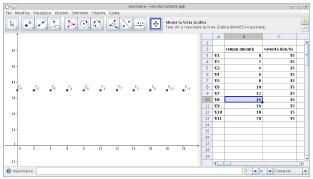
\includegraphics[width=.7\textwidth]{../immagini/velocitaCostante.jpeg}
 % podista.png
 %\label{fig:il grafico velocità tempo di un moto costante}
\end{figure}

Anche in questo caso, dai punti sperimentali è possibile derivare una retta, che risulta rigorosamente parallela all’asse dei tempi. Ma a noi interessa il modo in cui ` possibile ricavare informazione sullo spostamento dell’oggetto in movimento. Siccome, per definizione, la velocità di un moto costante è uguale allo spazio percorso diviso per il tempo impiegato, possiamo dedurre, a rovescio che, conoscendo la velocità e l’intervallo di tempo, si possa ricavare lo spazio da una moltiplicazione:
\begin{center}
\begin{math}
\Delta s = v * \Delta t 
\end{math}
\end{center}

Guardando bene la figura seguente, si può aggiungere anche un’importante osservazione di carattere grafico: il prodotto della velocità per l’intervallo di tempo è uguale all’area di un rettangolo.
\begin{figure}[H]
 \centering
 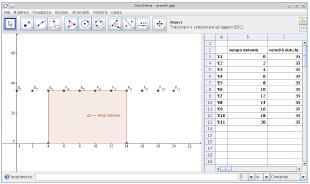
\includegraphics[width=.7\textwidth]{../immagini/spazioSottoIlGrafico_v-t.jpeg}
 % podista.png
 %\label{fig:il grafico velocità tempo di un moto costante}
\end{figure}

Bisogna fare attenzione a valutare correttamente l’informazione ricavabile da un grafico spazio tempo. La quantità definita spazio percorso, infatti, va distinta con attenzione dal concetto di posizione. Bisogna ribadire, infatti, che lo spazio percorso è definito come la differenza tra la posizione finale e la posizione iniziale.

Conoscendo, solo lo spazio percorso, non sarà perciò possibile individuare la posizione finale di un oggetto in movimento.
Alle volte, tuttavia, oltre allo spazio percorso, è possibile conoscere anche la posizione iniziale, e in questi casi risulta:
\begin{center}
\begin{math}
s_{finale} = s_{iniziale} + \Delta s = s_{iniziale} + v \Delta t
\end{math}
\end{center}
